%!TEX TS-program = xelatex
%!TEX encoding = UTF-8 Unicode
% Awesome CV LaTeX Template for CV/Resume
%
% This template has been downloaded from:
% https://github.com/posquit0/Awesome-CV
%
% Author:
% Claud D. Park <posquit0.bj@gmail.com>
% http://www.posquit0.com
%
% Template license:
% CC BY-SA 4.0 (https://creativecommons.org/licenses/by-sa/4.0/)
%


%-------------------------------------------------------------------------------
% CONFIGURATIONS
%-------------------------------------------------------------------------------
% A4 paper size by default, use 'letterpaper' for US letter
\documentclass[11pt, a4paper]{awesome-cv}

% Configure page margins with geometry
\geometry{left=1.8cm, top=1.5cm, right=1.8cm, bottom=2cm, footskip=.5cm}

% Specify the location of the included fonts
\fontdir[fonts/]

% Color for highlights
% Awesome Colors: awesome-emerald, awesome-skyblue, awesome-red, awesome-pink, awesome-orange
%                 awesome-nephritis, awesome-concrete, awesome-darknight
% \colorlet{awesome}{awesome-red}
% Uncomment if you would like to specify your own color
\definecolor{awesome}{HTML}{291185}

% Colors for text
% Uncomment if you would like to specify your own color
% \definecolor{darktext}{HTML}{414141}
% \definecolor{text}{HTML}{333333}
% \definecolor{graytext}{HTML}{5D5D5D}
% \definecolor{lighttext}{HTML}{999999}

% Set false if you don't want to highlight section with awesome color
\setbool{acvSectionColorHighlight}{false}

% If you would like to change the social information separator from a pipe (|) to something else
\renewcommand{\acvHeaderSocialSep}{\quad\textbar\quad}


%-------------------------------------------------------------------------------
%	PERSONAL INFORMATION
%	Comment any of the lines below if they are not required
%-------------------------------------------------------------------------------
% Available options: circle|rectangle,edge/noedge,left/right
% \photo[circle,noedge,left]{./contents/profile.png} % TODO UNCOMMENT
\name{Valentin}{Lucet}
\position{Ecologist{\enskip\cdotp\enskip}Research Software Engineer}
% \address{42-8, Bangbae-ro 15-gil, Seocho-gu, Seoul, 00681, Rep. of KOREA}

\mobile{(+1) 438-832-5167}
\email{Valentin.lucet@gmail.com}
%\dateofbirth{January 1st, 1970}
\homepage{vlucet.github.io}
\github{vlucet}
\linkedin{valentin-lucet}
% \gitlab{gitlab-id}
% \stackoverflow{SO-id}{SO-name}
\twitter{VLucet}
% \skype{skype-id}
% \reddit{reddit-id}
% \medium{medium-id}
\googlescholar{cIHIw5IAAAAJ}{V. Lucet}
%% \firstname and \lastname will be used
% \googlescholar{googlescholar-id}{}
% \extrainfo{extra information}

\quote{As an ecologist, I am interested in complex working landscapes, social ecological systems, and interdisciplinary approaches.
\\ Passionate about open and reproducible science, I develop tools for researchers and managers, and teach computational methods.}


%-------------------------------------------------------------------------------
\begin{document}

% Print the header with above personal information
% Give optional argument to change alignment(C: center, L: left, R: right)
\makecvheader

% Print the footer with 3 arguments(<left>, <center>, <right>)
% Leave any of these blank if they are not needed
\makecvfooter
  {\today}
  {V. Lucet~~~·~~~CV}
  {\thepage}


%-------------------------------------------------------------------------------
%	CV/RESUME CONTENT
%	Each section is imported separately, open each file in turn to modify content
%-------------------------------------------------------------------------------
% !TeX root = ../cv.tex

\cvsection{Education}

\begin{cventries}
	
	\cventry
	{M.SC. IN PHYSICS} % Degree
	{Universidade do Porto} % Institution
	{Porto, Portugal} % Location
	{Setp. 2015 - PRESENT} % Date(s)
	{
		\begin{cvitems} % Description(s) bullet points
			\item {Currently following the theoretical branch and taking some mathematics courses}
			\item {Current classification \textbf{17/20}}
		\end{cvitems}
	}
	
	\cventry
	{B.S. IN PHYSICS} % Degree 
	{Universidade do Porto} % Institution
	{Porto, Portugal} % Location
	{Sept. 2011 - Jul. 2015} % Date(s)
	{
		\begin{cvitems} % Description(s) bullet points
			\item {National classification \textbf{17/20}, post-Bologna}
			\item {Minor in Physics}
		\end{cvitems}
	}
	
	\cventry
	{{\normalsize 12}TH GRADE} % Degree 
	{Agrupamento Vertical de Escolas de Ponte da Barca} % Institution
	{Ponte da Barca, Portugal} % Location
	{Sept. 2008 - Jul. 2011} % Date(s)
	{
		\begin{cvitems} % Description(s) bullet points
			\item {National classification \textbf{18/20}}
			%\item {Main subjects: \emph{Mathematics, Portuguese, English, Physics, Chemistry, Biology, Geology}}
		\end{cvitems}
	}
	
\end{cventries}

%-------------------------------------------------------------------------------
%	SECTION TITLE
%-------------------------------------------------------------------------------
\vspace{-20pt}
\cvsection{Skills}


%-------------------------------------------------------------------------------
%	CONTENT
%-------------------------------------------------------------------------------
\begin{cvskills}

%---------------------------------------------------------
  \cvskill
    {Programming} % Category
    {R (advanced) / Python, Julia, Bash, SQL, Matlab (familiar)} % Skills

%---------------------------------------------------------
  \cvskill
    {GIS tools} % Category
    {GDAL, GRASS, QGIS, ArcGIS (proficient) - PostGIS (familiar)} % Skills

%---------------------------------------------------------
  \cvskill
    {Other} % Category
    {Git \& GitHub (incl. pages), Docker, Markdown, LaTex, Hugo} % Skills

%---------------------------------------------------------
  \cvskill
    {Languages} % Category
    {French (native) - English (fluent) - Spanish (basics)} % Skills

%---------------------------------------------------------
\end{cvskills}

%-------------------------------------------------------------------------------
%	SECTION TITLE
%-------------------------------------------------------------------------------
\vspace{3pt}
\cvsection{Experience}

\vspace{-2pt}
%-------------------------------------------------------------------------------
%	CONTENT
%-------------------------------------------------------------------------------
\begin{cventries}

%---------------------------------------------------------
  \cventry
    {Concordia University - Pedersen Quantitative Fisheries Ecology Lab} % Organization
    {Research Software Developer} % Job title
    {Montreal, QC} % Location
    {2021 - Present} % Date(s)
    {
      \begin{cvitems} % Description(s) of tasks/responsibilities
        \item {Development of the \textbf{sspm} and \textbf{csdm} R packages, workshop development and delivery with DFO}
        \item {Grad student mentoring: teaching of skills for open and reproducible science}
      \end{cvitems}
    }

%---------------------------------------------------------
  \cventry
  {Environment and Climate Change Canada ~·~ Landscape Science Unit} % Organization
  {Data Scientist} % Job title
  {QC} % Location
  {2021 - 2021} % Date(s)
  {
    \begin{cvitems} % Description(s) of tasks/responsibilities
      \item {Contributions to R packages \textbf{pfocal} and \textbf{LSTDConnect} (currently private)}
      \item {Contributions to a Canada-wide connectivity analysis (in prep)}
    \end{cvitems}
  }

  %---------------------------------------------------------
  \cventry
  {APEX Resources Management Solutions} % Organization
  {Landscape ecologist} % Job title
  {QC} % Location
  {2020 - 2021} % Date(s)
  {
    \begin{cvitems} % Description(s) of tasks/responsibilities
      \item {Projects: carbon cycle models, epidemiological models, \textbf{STSIM} development and maintenance}
    \end{cvitems}
  }

%---------------------------------------------------------
\end{cventries}

\vspace{-6pt}
\cvsubsection{Contracts \& Consulting}

\begin{cventries}

    %---------------------------------------------------------
    \cventry
    {R developper} % Job title
    {APEX Resources Management Solutions} % Organization
    {QC} % Location
    {2019 - 2020} % Date(s)
    {
      \begin{cvitems} % Description(s) of tasks/responsibilities
        \item {Improvement and CRAN submission for the R package \textbf{Rsyncrosim}}
      \end{cvitems}
    }

    %---------------------------------------------------------
    \cventry
    {Reporter} % Job title
    {MELCC – Ministère de l'Environnement} % Organization
    {QC} % Location
    {2019} % Date(s)
    {
      \begin{cvitems} % Description(s) of tasks/responsibilities
        \item {Contributions to an analysis of ecological connectivity for the Saint Lawrence Lowlands and translation to French}
      \end{cvitems}
    }

    %---------------------------------------------------------
    \cventry
    {Reporter} % Job title
    {MFFP – Ministère des Forêts, de la Faune et des Parcs} % Organization
    {QC} % Location
    {2019} % Date(s)
    {
      \begin{cvitems} % Description(s) of tasks/responsibilities
        \item {Contributions to a report on ecological connectivity in the northwest America as part of the working group related to the 40-3 resolution}
      \end{cvitems}
    }
  
\end{cventries}
% %-------------------------------------------------------------------------------
%	SECTION TITLE
%-------------------------------------------------------------------------------
\cvsection{Volunteering}


%-------------------------------------------------------------------------------
%	CONTENT
%-------------------------------------------------------------------------------
\begin{cventries}

%---------------------------------------------------------
  \cventry
    {\href{https://www.youtube.com/channel/UCPDmodXhx7DcY5j6-_ZjjKA/featured}{Fundraising Ambassador}} % Affiliation/role
    {\href{https://www.mcgill.ca/redpath/}{Redpath Museum}} % Organization/group
    {McGill University} % Location
    {2015 - 2017} % Date(s)
    {
      \begin{cvitems} % Description(s) of experience/contributions/knowledge
        \item {\href{https://www.mcgill.ca/seedsofchange/project/redpath-museum-plesiosaur}{Seeds of Change Plesiosaur project} - \$13,000 raised}
        \item {\href{https://www.mcgill.ca/seedsofchange/project/cutting-edge-lecture-series-project}{Seeds of Change Cutting Edge Lectures project} - \$2,850 raised}
      \end{cvitems}
    }

%---------------------------------------------------------
  \cventry
    {VP Communications, VP events, VP} % Affiliation/role
    {\href{https://redpathmuseumsociety.weebly.com/}{Redpath Museum Student Society}} % Organization/group
    {McGill University} % Location
    {2015-2018} % Date(s)
    {}

%---------------------------------------------------------
  \vspace{-8pt}
  \cventry
    {Morning Survey Volunteer for a total of 5 months} % Affiliation/role
    {\href{https://www.archelon.gr/index_eng.php}{ARCHELON (Sea Turtle Protection Society of Greece)}} % Organization/group
    {Crete} % Location
    {2015, 2016} % Date(s)
    {}

%---------------------------------------------------------
  \vspace{-8pt}
  \cventry
    {Undergraduate Volunteer} % Affiliation/role
    {\href{https://www.abouheiflab.org/}{Abouheif Lab}} % Organization/group
    {McGill University} % Location
    {2015-2016} % Date(s)
    {}

%---------------------------------------------------------
  \vspace{-8pt}
  \cventry
    {Public awareness volunteer} % Affiliation/role
    {\href{https://wwf.ca/fr/stories/projet-ours-polaire-limpact-du-rechauffement-sur-les-populations-du-nord/}{WWF Quebec - Project “Ours Polaire sur Glaces Ephémères}} % Organization/group
    {Montreal, QC} % Location
    {2015} % Date(s)
    {}

%---------------------------------------------------------
  \vspace{-8pt}
  \cventry
    {Morning Survey Volunteer} % Affiliation/role
    {\href{https://www.oommbo.org/}{McGill bird observatory}} % Organization/group
    {Montreal, QC} % Location
    {2014} % Date(s)
    {}

%---------------------------------------------------------
  \vspace{-8pt}
  \cventry
    {Intern - Manuscript proof reader} % Affiliation/role
    {\href{https://www.editis.com/maisons/eho/}{Editions Heloise D’Ormesson}} % Organization/group
    {Paris, France} % Location
    {2012} % Date(s)
    {}

%---------------------------------------------------------
\end{cventries}
\vspace{-12pt}
%-------------------------------------------------------------------------------
%	SECTION TITLE
%-------------------------------------------------------------------------------
\cvsection{Software}

%-------------------------------------------------------------------------------
%	CONTENT
%-------------------------------------------------------------------------------
\begin{table}[h!]
  \footnotesize
  \begin{center}
  \begin{tabular}{c  c  c | c | c  c}
  \multicolumn{3}{c}{\textbf{Cre.}} & \multicolumn{1}{c}{\textbf{Aut.}} & \multicolumn{2}{c}{\textbf{Ctb.}} \\
  \href{https://github.com/vlucet/rgovcan}{\textit{rgovcan}} & 
  \href{https://github.com/vlucet/rgrassdoc}{\textit{rgrassdoc}} & 
  \href{https://github.com/pedersen-fisheries-lab/sspm}{\textit{rgeobon}} &
  \href{https://github.com/pedersen-fisheries-lab/sspm}{\textit{sspm}} &
  \href{https://github.com/syncrosim/rsyncrosim}{\textit{rsyncrosim}} &
  \href{https://github.com/simonmoulds/lulcc}{\textit{lulcc}}\\ 
  \raisebox{-\totalheight}{
\includegraphics[scale=0.4]{pkgs/rgovcan.png}} & 
  \raisebox{-\totalheight}{
\includegraphics[scale=0.4]{pkgs/rgrassdoc.png}} &
  \raisebox{-\totalheight}{
\includegraphics[scale=0.4]{pkgs/rgeobon.png}} &
  \raisebox{-\totalheight}{
\includegraphics[scale=0.4]{pkgs/sspm.png}} &
  \raisebox{-\totalheight}{
\includegraphics[scale=0.4]{pkgs/rsyncrosim.png}} &
  \raisebox{-\totalheight}{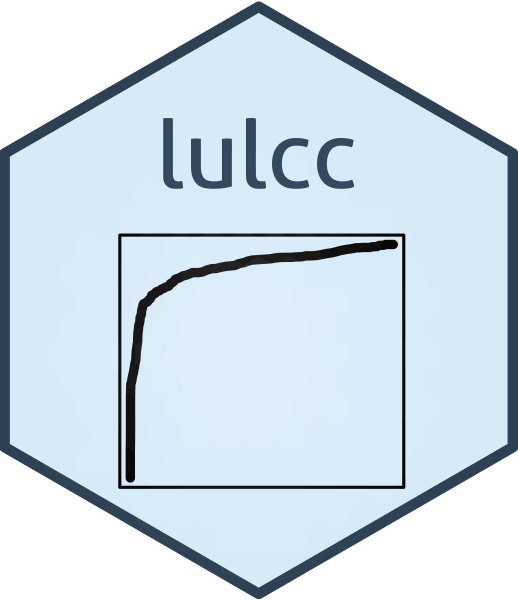
\includegraphics[scale=0.4]{pkgs/lulcc.png}}\\
  \end{tabular}
  \end{center}
\end{table}

% !TeX root = ../cv.tex
%-------------------------------------------------------------------------------
%	SECTION TITLE
%-------------------------------------------------------------------------------
\vspace{5pt}
\cvsection{Honors \& Awards}

%-------------------------------------------------------------------------------
%	CONTENT
%-------------------------------------------------------------------------------
\begin{cvhonors}

%---------------------------------------------------------
  \cvhonor
    {QCBS Learning and Development Award} % Award
    {} % Event
    {\$150} % Location
    {2021} % Date(s)

%---------------------------------------------------------
  \cvhonor
    {QCBS Excellence Travel Award} % Award
    {} % Event
    {Waived (COVID-19)} % Location
    {2020} % Date(s)

%---------------------------------------------------------
  \cvhonor
    {FRQNT (Fonds de Recherche du Québec - Nature et Technologie) M.Sc. Bursary} % Award
    {} % Event
    {\$17,5k} % Location
    {2019} % Date(s)

%---------------------------------------------------------
  \cvhonor
    {Frank Rigler Prize in Ecology} % Award
    {} % Event
    {\$785} % Location
    {2018} % Date(s)

%---------------------------------------------------------
  \cvhonor
    {SURA (Student Undergraduate Research Award)} % Award
    {} % Event
    {\$6,725} % Location
    {2017} % Date(s)
    
    % "Dean's Honour List", "2015", "" 
    % "Grad Excellence Award", "2019", "2,500",

%---------------------------------------------------------
\end{cvhonors}
\vspace{20pt}
%-------------------------------------------------------------------------------
%	SECTION TITLE
%-------------------------------------------------------------------------------
\cvsection{Presentation}


%-------------------------------------------------------------------------------
%	CONTENT
%-------------------------------------------------------------------------------
\begin{cventries}

%---------------------------------------------------------
  \cventry
    {Presenter for <DEFCON 20th : The way to go to Las Vegas>} % Role
    {6th CodeEngn (Reverse Engineering Conference)} % Event
    {Seoul, S.Korea} % Location
    {Jul. 2012} % Date(s)
    {
      \begin{cvitems} % Description(s)
        \item {Introduced CTF(Capture the Flag) hacking competition and advanced techniques and strategy for CTF}
      \end{cvitems}
    }

%---------------------------------------------------------
  \cventry
    {Presenter for <Metasploit 101>} % Role
    {6th Hacking Camp - S.Korea} % Event
    {S.Korea} % Location
    {Sep. 2012} % Date(s)
    {
      \begin{cvitems} % Description(s)
        \item {Introduced basic procedure for penetration testing and how to use Metasploit}
      \end{cvitems}
    }

%---------------------------------------------------------
\end{cventries}

%-------------------------------------------------------------------------------
%	SECTION TITLE
%-------------------------------------------------------------------------------
\cvsection{Writing}


%-------------------------------------------------------------------------------
%	CONTENT
%-------------------------------------------------------------------------------
\begin{cventries}

%---------------------------------------------------------
  \cventry
    {Founder \& Writer} % Role
    {A Guide for Developers in Start-up} % Title
    {Facebook Page} % Location
    {Jan. 2015 - PRESENT} % Date(s)
    {
      \begin{cvitems} % Description(s)
        \item {Drafted daily news for developers in Korea about IT technologies, issues about start-up.}
      \end{cvitems}
    }

%---------------------------------------------------------
  \cventry
    {Undergraduate Student Reporter} % Role
    {AhnLab} % Title
    {S.Korea} % Location
    {Oct. 2012 - Jul. 2013} % Date(s)
    {
      \begin{cvitems} % Description(s)
        \item {Drafted reports about IT trends and Security issues on AhnLab Company magazine.}
      \end{cvitems}
    }

%---------------------------------------------------------
\end{cventries}

% %-------------------------------------------------------------------------------
%	SECTION TITLE
%-------------------------------------------------------------------------------
\cvsection{Program Committees}


%-------------------------------------------------------------------------------
%	CONTENT
%-------------------------------------------------------------------------------
\begin{cvhonors}

%---------------------------------------------------------
  \cvhonor
    {Problem Writer} % Position
    {2016 CODEGATE Hacking Competition World Final} % Committee
    {S.Korea} % Location
    {2016} % Date(s)

%---------------------------------------------------------
  \cvhonor
    {Organizer \& Co-director} % Position
    {1st POSTECH Hackathon} % Committee
    {S.Korea} % Location
    {2013} % Date(s)

%---------------------------------------------------------
  \cvhonor
    {Staff} % Position
    {7th Hacking Camp} % Committee
    {S.Korea} % Location
    {2012} % Date(s)

%---------------------------------------------------------
  \cvhonor
    {Problem Writer} % Position
    {1st Hoseo University Teenager Hacking Competition} % Committee
    {S.Korea} % Location
    {2012} % Date(s)

%---------------------------------------------------------
  \cvhonor
    {Staff \& Problem Writer} % Position
    {JFF(Just for Fun) Hacking Competition} % Committee
    {S.Korea} % Location
    {2012} % Date(s)

%---------------------------------------------------------
\end{cvhonors}


%-------------------------------------------------------------------------------
\end{document}
